\section{Twisted representation via a sublattice}\label{S:sublattice}

\subsection{Sublattices and subalgebras}

Consider a full rank sublattice $\Lambda \subset \mathbb{Z}^2$ of index $n$ (i.e., $\mathbb{Z}^2/\Lambda$ is a finite group of order $n$). Let us define a Lie subalgebra $\qD^{\Lambda} \subset \qD$ which is spanned by $E_{a,b}$ for $(a,b) \in \Lambda$ and central elements~$c$,~$c'$.

Denote by $E_{a,b}^{[n]}$, $c_{[n]}$, $c'_{[n]}$ standard generators of $\qDn$. Let $v_1 = (k_1, l_1)$ and $v_2 = (k_2, l_2)$ be a basis of $\Lambda$. Define a map $\varphi_{v_1, v_2}\colon \qDn \rightarrow \qD$
\begin{gather*}
\varphi_{v_1, v_2} E^{\scriptstyle{[n]}}_{a,b} = E_{a k_1 + b k_2, a l_1 + b l_2}, \qquad
\varphi_{v_1, v_2} c'_{\scriptstyle{[n]}} = k_1 c' + l_1 c, \qquad
\varphi_{v_1, v_2} c_{\scriptstyle{[n]}} = k_2 c' + l_2 c.
\end{gather*}

\begin{Proposition}
Let $v_1$, $v_2$ be a positively oriented basis $($i.e., $k_1 l_2 - k_2 l_1 =n)$. Then the map~$\varphi_{v_1, v_2}$ is a Lie algebra isomorphism $\qDn \cong \qD^{\Lambda}$.
\end{Proposition}

\begin{proof}It follows from \eqref{qDc} directly.
\end{proof}

Slightly abusing notation, denote the Fock representation of $\qDn$ by $\mathcal{F}_u^{[n]}$ .

\begin{Proposition} \label{LambdaFock}
Let $v_1 = (n,0)$ and $v_2 =(-m, 1)$. Then $ \mathcal{F}_{u^{n}}^{[n]} \cong \left. \mathcal{F}_u \right|_{\phi_{v_1, v_2} \left(\qd{n} \right)}$ as $\qd{n}$-modules.
\end{Proposition}

\begin{proof}
Note that the Fock module $\mathcal{F}_u$ is $\mathbb{Z}$-graded with grading given by
\begin{gather*}
\deg(| \alpha \rangle) = 0, \qquad \deg (E_{a,b})=-b.
\end{gather*}
Recall that a character of a $\mathbb{Z}$-graded module is the generating function of dimensions of the graded components. Then the character of Fock module $\ch \mathcal{F}_u = 1/(\mathfrak{q})_{ \infty } := \prod\limits_{k=1}^{\infty} 1/\big(1-\mathfrak{q}^k\big)$.

Consider a subalgebra $\Hem_0$ in $\qd{n}$ spanned by $E_{0, k}$ and $c$. Note that $\Hem_0$ is isomorphic to the Heisenberg algebra. Since $\deg (\phi_{v_1,v_2}E_{0,-k} )= \deg (E_{km,-k}) = k$, the character of the $\Hem_0$-Fock module is also $1/(\mathfrak{q})_{\infty}$; i.e., it coincides with $\ch \mathcal{F}_u$. This implies that $\left. \mathcal{F}_u \right|_{\phi_{v_1, v_2} \left(\qd{n} \right)}$ restricted to $\Hem_0$ is isomorphic to the $\Hem_0$-Fock module. To finish the proof, we use Propositions \ref{Fock} and \ref{E_l}.
\end{proof}

\subsection{Twisted Fock vs restricted Fock}
From now on we change $q \rightarrow q^{1/n}$.
Our goal is to construct an action of $\qD$ on the Fock module twisted by $\sigma \in {\rm SL}_2 ( \mathbb{Z} )$ as in \eqref{sigma} for $n \neq 0$. Consider a sublattice $\Lambda_{\sigma} \subset \mathbb{Z}^2$ spanned by $v_1 = (n,0)$ and $v_2 = (-m, 1)$. Consider another basis of $\Lambda_{\sigma}$ obtained by $\sigma$
\begin{gather}
w_1= m' v_1 + n' v_2 = (m' n - n' m, n') = (1, n'), \label{eq: v to w change 1} \\
w_2= m v_1 + n v_2 = (0, n). \label{eq: v to w change 2}
\end{gather}

\begin{figure}[t]\centering
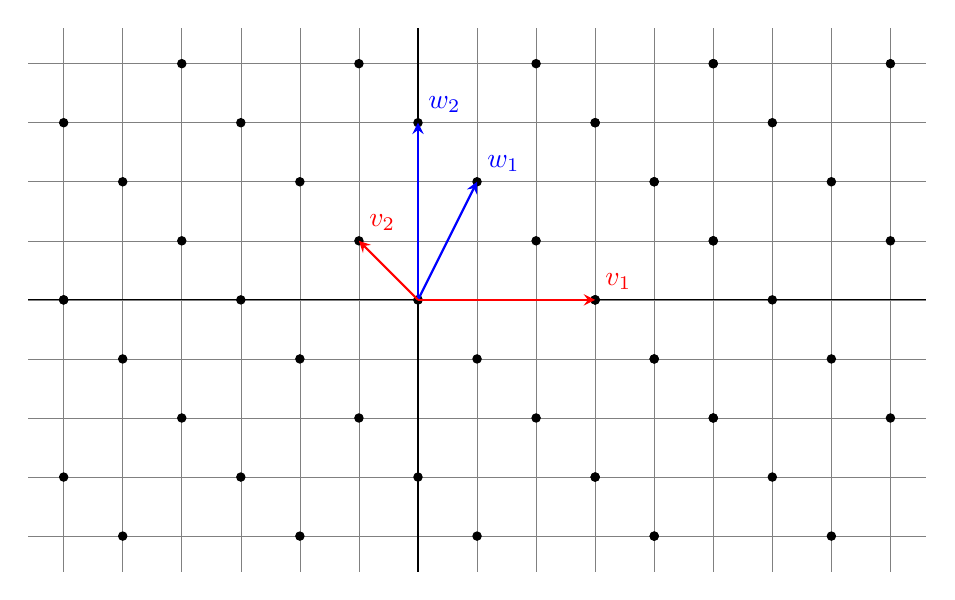
\begin{tikzpicture}[scale=1.5]
\draw[step=.5cm,gray,very thin] (-3.3,-2.3) grid (4.3,2.3);
\draw[thin] (-3.3,0) -- (4.3,0);
\draw[thin] (0,-2.3) -- (0,2.3);
\foreach \point in {(-3,0),(0,0),(1.5,0)}
{
\draw[fill] \point circle (1pt);
\draw[fill] \point+(1.5,0) circle (1pt);
\draw[fill] \point circle (1pt);
\draw[fill] \point+(1,0.5) circle (1pt);
\draw[fill] \point+(2.5,0.5) circle (1pt);
\draw[fill] \point+(0.5,1) circle (1pt);
\draw[fill] \point+(2,1) circle (1pt);
\draw[fill] \point+(0,1.5) circle (1pt);
\draw[fill] \point+(1.5,1.5) circle (1pt);\draw[fill] \point+(0,-1.5) circle (1pt);
\draw[fill] \point+(1.5,-1.5) circle (1pt);
\draw[fill] \point+(1,-1) circle (1pt);
\draw[fill] \point+(2.5,-1) circle (1pt);
\draw[fill] \point+(0.5,-0.5) circle (1pt);
\draw[fill] \point+(2,-0.5) circle (1pt);
\draw[fill] \point+(1,2) circle (1pt);
\draw[fill] \point+(2.5,2) circle (1pt);
\draw[fill] \point+(0.5,-2) circle (1pt);
\draw[fill] \point+(2,-2) circle (1pt);
}
\draw[->,>=stealth,thick,blue] (0,0) to (0.5,1) node[anchor=south west] {$w_1$};
\draw[->,>=stealth,thick,blue] (0,0) to (0,1.5) node[anchor=south west] {$w_2$};
\draw[->,>=stealth,thick,red] (0,0) to (1.5,0) node[anchor=south west] {$v_1$};
\draw[->,>=stealth,thick,red] (0,0) to (-0.5,0.5) node[anchor=south west] {$v_2$};
\end{tikzpicture}
\caption{Lattice $\Lambda_\sigma$ for $n=3$, $m=1$.}\label{fig:Lambda_sigma}
\end{figure}

\begin{Remark}
The construction of the sublattice $\Lambda_{\sigma} \subset \mathbb{Z}^2$ naturally appears, if one require $\sigma$ to be a transition matrix from $v_i$ to $w_i$ and assume $v_1 = (n, 0)$, $w_2 = (0, n)$.
\end{Remark}

Denote the Fock module of $\qd{1/n}$ by $\mathcal{F}^{[1/n]}_{u}$.

\begin{Theorem}\label{MainTh}There is an isomorphism of $\qD$-modules $\left. ( \mathcal{F}_{u})^{ \sigma } \cong \mathcal{F}^{[1/n]}_{u^{1/n}} \right|_{\phi_{w_1,w_2} (\qD) }$.
\end{Theorem}

\begin{proof}Proposition \ref{LambdaFock} implies $\left. \mathcal{F}^{[1/n]}_{u^{1/n}} \right|_{\phi_{v_1,v_2}(\qD)} \cong \mathcal{F}_{u}$. On the other hand, relations~\eqref{eq: v to w change 1} and~\eqref{eq: v to w change 2} yield that $\sigma$ is the transition matrix from $w_1$, $w_2$ to $v_1$, $v_2$.
\end{proof}

\begin{Corollary}There is an isomorphism of $\qD$-modules $\left. ( \mathcal{M}_{u} )^{ \sigma } \cong \mathcal{M}^{[1/n]}_{u^{1/n}} \right|_{\phi_{w_1,w_2} (\qD ) }$.
\end{Corollary}

Theorem \ref{MainTh} combined with results from Section \ref{level1} enables us to find explicit formulas for action on $\mathcal{F}_{u}^{ \sigma }$. We will do this below.

\subsection{Explicit formulas for restricted Fock}
\subsubsection{Fermionic construction via sublattice}
Denote fermionic representation of $\qd{1/n}$ by $\mathcal{M}^{[1/n]}_u$. To be more specific, let us rewrite formulas from Section~\ref{fermi} for $\mathcal{M}^{[1/n]}_{u^{1/n}}$.
\begin{align}
&c \mapsto 1, \qquad c' \mapsto 0, \qquad H_m \rightarrow \sum_{i+j=m} \psi_i \psi_j^*, \nonumber\\
&E(z) \mapsto \frac{q^{l/n} u^{1/n} }{1-q^{1/n}} + u^{1/n} q^{ - 1/2n }z : \! \psi\big( q^{-1/2n} z\big) \psi^* \big( q^{1/2n} z\big) \! :_{(l)} ,
\label{ferm:En} \\
&F(z) \mapsto \frac{q^{-l/n} u^{-1/n} }{1-q^{-1/n}} + u^{-1/n} q^{1/2n} z : \! \psi\big( q^{1/2n} z\big) \psi^* \big(q^{-1/2n} z\big)\!:_{(l)}.
\label{ferm:Fn}
\end{align}
\begin{Proposition} \label{TheFermionicProp}
The following formulas below determine an action of $\qD$ on $F^{n\psi}$
\begin{gather}
c=n, \qquad c' = n_{tw}, \qquad
H^{tw}_k = \sum_{a} \sum_{i+j=k} \psi_a [i] \psi^*_a [j] , \label{eq1: TheFermionicProp} \\
E^{tw}(z) = \sum_{b-a \equiv -n_{tw} \bmod n} u^{\frac{1}{n}} q^{-1/2} z \psia \big( q^{-1/2} z\big) \psib \big(q^{1/2} z\big) z^{\frac{n_{tw}-a+b}{n}} q^{(a+b)/2n}, \label{prop:EtwFermi} \\
F^{tw}(z) = \sum_{b-a \equiv n_{tw} \bmod n} u^{-\frac{1}{n}} q^{1/2} z \psia \big( q^{1/2} z\big) \psib \big(q^{-1/2} z\big) z^{\frac{-n_{tw}-a+b}{n}} q^{-(a+b)/2n}. \label{prop:FtwFermi}
\end{gather}
The module obtained is isomorphic to $\left. \mathcal{M}^{[1/n]}_{u^{1/n}} \right|_{\phi_{w_1, w_2}(\qD)}$ for $w_1=(1, n_{tw})$, $w_2=(0,n)$.
\end{Proposition}

\begin{Remark}
Below we will substitute $n_{tw}=n'$ to prove Theorem \ref{TheFermionicTh}. However, Proposi\-tion~\ref{TheFermionicProp} is more general, than it is necessary for the proof, since we do not assume here that $\gcd(n, n_{tw})=1$. We will need the case of arbitrary $n_{tw}$ in Section~\ref{Section: general sublattice}.
\end{Remark}

\begin{proof}
We use the notation $E(z)$, $F(z)$ and $H(z)$ for the Chevalley generators of $\mathfrak{Diff}_{q^{1/n}}$. The generators of $\qD \cong \mathfrak{Diff}_{q^{1/n}}^{\Lambda}$ (identified by $\varphi_{w_1,w_2}$) will be denoted by $E^{tw}(z)$, $F^{tw}(z)$ and $H^{tw} (z)$. Let us write the identification $\phi_{w_1,w_2}$ explicitly for the Chevalley generators
\begin{gather}
H^{tw}(z) = \sum_k H_{ 0, nk} z^{-k}, \label{eq: tw chevalleyH}\\
E^{tw}(z) = z^{n_{tw}/n} \sum_{k \equiv n_{tw} \bmod n} E_{k} z^{-k/n}, \\
F^{tw}(z) = z^{-n_{tw}/n} \sum_{k \equiv -n_{tw} \bmod n} F_{ k} z^{-k/n} .\label{eq: tw chevalleyF}
\end{gather}

Let us consider currents $\psia (z)$ and $\psib (z)$ for $a,b = 0, 1, \dots, n-1$. These currents are defined by following equality
\begin{gather}
z \psi(z) = \sum_{a=0}^{n-1} z^{n-a} \psia (z^n) , \qquad
\psi^*(z) = \sum_{b=0}^{n-1} z^{b} \psib (z^n).\label{defa1}
\end{gather}
Let us denote the modes of $\psia (z)$ and $\psib (z)$ as in equality~\eqref{eq:nFermions}. It is easy to see that these modes satisfy Clifford algebra relations \eqref{eq:nClifford1}, \eqref{eq:nClifford2}. So we have identified the Clifford algebra and the $n$th power of Clifford algebra. This leads to an identification $F^{\psi}=F^{n \psi}$.

Substituting \eqref{defa1} into \eqref{ferm:En} and \eqref{ferm:Fn}, we obtain
\begin{gather*}
E(z) = \frac{q^{l/n} u^{1/n} }{1-q^{1/n}} + \sum_{a=0}^{n-1} \sum_{b=0}^{n-1} u^{1/n} q^{\frac{a+b}{2n}} q^{-1/2} z^{n-a+b} : \! \psia \big( q^{-1/2} z^n\big) \psib \big(q^{1/2} z^n\big) \! :_{(l)}, \\
F(z) = \frac{q^{-l/n} u^{-1/n} }{1-q^{-1/n}} + \sum_{a=0}^{n-1} \sum_{b=0}^{n-1} u^{-1/n} q^{- \frac{a+b}{2n}} q^{1/2} z^{n-a+b} : \! \psia \big( q^{1/2} z^n \big) \psib \big(q^{-1/2} z^n \big)\!:_{(l)}.
\end{gather*}
For technical reasons, we need to treat the cases $n_{tw} \neq 0$ and $n_{tw} =0$ separately. Let us first consider the case $n_{tw} \neq 0$. Using formulas \eqref{eq: tw chevalleyH}--\eqref{eq: tw chevalleyF}, we see that
\begin{gather*}
E^{tw}(z) = \sum_{a-b \equiv n_{tw} \bmod n} \! \! q^{\frac{a+b}{2n}} u^{1/n} z^{\frac{n_{tw}-a+b}{n}} q^{-1/2} z \psia \big( q^{-1/2} z\big) \psib \big(q^{1/2} z\big), \\
F^{tw} (z) = \sum_{a-b \equiv -n_{tw} \bmod n} \! \!q^{\frac{-(a+b)}{2n}} u^{-1/n} z^{\frac{-n_{tw}-a+b}{n}} q^{1/2} z \psia \big( q^{1/2} z \big) \psib \big(q^{-1/2} z \big) .
\end{gather*}
For $n_{tw}=0$ we obtain
\begin{gather*}
E^{tw}(z) = \frac{q^{l/n} u^{1/n} }{1-q^{1/n}} + \sum_{a=0}^{n-1} u^{1/n} q^{a/n} q^{-1/2} z : \! \psia \big( q^{-1/2} z\big) \psiaa \big(q^{1/2} z\big) \! :_{(l)}, \\
F^{tw}(z) = \frac{q^{-l/n} u^{-1/n} }{1-q^{-1/n}} + \sum_{a=0}^{n-1} u^{-1/n} q^{-a/n} q^{1/2} z : \! \psia \big( q^{1/2} z \big) \psiaa \big(q^{-1/2} z \big)\!:_{(l)}.
\end{gather*}
This can be rewritten as
\begin{gather*}
E^{tw}(z) = \sum_{a=0}^{n-1} u^{1/n} q^{a/n} \left( \frac{q^{ \ceil{\frac{l-a}{n}} }}{1-q} +q^{-1/2} z : \! \psia \big( q^{-1/2} z\big) \psiaa \big(q^{1/2} z\big) \! :_{(l)} \right), \\
F^{tw}(z) = \sum_{a=0}^{n-1} u^{-1/n} q^{-a/n} \left( \frac{q^{- \ceil{\frac{l-a}{n}} }}{1-q^{-1}} + q^{1/2} z : \! \psia \big( q^{1/2} z \big) \psiaa \big(q^{-1/2} z \big)\!:_{(l)} \right) .
\end{gather*}
Note that the $l$-dependent normal ordering is defined in terms of $\psi_i$ and $\psi^*_j$. One can check (cf.~\eqref{eq: regul prod psipsi})
\begin{align} \label{eq: psia OPE}
\psia(z) \psiaa(w) = \frac{(w/z)^{\ceil{\frac{l-a}{n}} }}{z(1-w/z)} + : \! \psia (z) \psiaa (w) \! :_{(l)}.
\end{align}
Hence
\begin{equation*}
q^{-1/2} z \psia\big(q^{-1/2}z\big) \psiaa\big(q^{1/2}z\big) = \frac{q^{\ceil{\frac{l-a}{n}} }}{1-q} + q^{-1/2} z : \! \psia \big(q^{-1/2}z\big) \psiaa \big(q^{1/2}z\big) \! :_{(l)}.\tag*{\qed}
\end{equation*}\renewcommand{\qed}{}
\end{proof}

\begin{proof}[Proof of Theorem \ref{TheFermionicTh}] Follows from Theorem \ref{MainTh} and Proposition \ref{TheFermionicProp}.
\end{proof}
